\documentclass[12pt,a4paper,twoside,openright,italian]{book} % PER ITALIANO
%\documentclass[12pt,a4paper,twoside,openright,english]{book} % PER INGLESE
\pagestyle{plain}

\usepackage[italian]{babel} %PER ITALIANO
%\usepackage[english]{babel} %PER INGLESE
\usepackage[T1]{fontenc}
%\usepackage[latin9]{inputenc} % PER WINDOWS
\usepackage[utf8]{inputenc} % PER LINUX


\usepackage{url}
\usepackage{amsmath}
\usepackage{graphicx}
\usepackage{setspace}
\usepackage{amssymb}
\usepackage{hyperref}
\usepackage{color}
\usepackage{graphicx}
\usepackage{multicol}
\usepackage {fancyhdr}
\usepackage{geometry}
\usepackage{natbib}
\usepackage{lipsum}
\usepackage[labelfont={normalfont, bf}, font=it]{caption}
\usepackage{blindtext}
\usepackage[lined,boxed,commentsnumbered,linesnumbered]{algorithm2e}
\usepackage{listings}
\usepackage{color}
\renewcommand{\ttdefault}{cmtt}

\usepackage[dvipsnames]{xcolor} % colori
\usepackage[lighttt]{lmodern}

\usepackage{bchart}

\usepackage{wrapfig}

\usepackage[lf]{Baskervaldx} % lining figures
\usepackage[bigdelims,vvarbb]{newtxmath} % math italic letters from Nimbus Roman
\usepackage[cal=boondoxo]{mathalfa} % mathcal from STIX, unslanted a bit

\usepackage{subcaption} %consente le didascalie per più immagini affiancate


\usepackage{color}
\definecolor{gray}{rgb}{0.4,0.4,0.4}
\definecolor{darkblue}{rgb}{0.0,0.0,0.6}
\definecolor{cyan}{rgb}{0.0,0.6,0.6}

\lstset{
  basicstyle=\ttfamily,
  columns=fullflexible,
  showstringspaces=false,
  commentstyle=\color{gray}\upshape
}

\lstdefinelanguage{XML}
{
  morestring=[b]",
  morestring=[s]{>}{<},
  morecomment=[s]{<?}{?>},
  stringstyle=\color{black},
  identifierstyle=\color{darkblue},
  keywordstyle=\color{cyan},
  morekeywords={xmlns,version,type}% list your attributes here
}

\lstdefinelanguage{JSON}
{
  morestring=[b]",
  morestring=[s]{>}{<},
  stringstyle=\color{darkblue},
  identifierstyle=\color{darkblue},
  keywordstyle=\color{cyan},
  morekeywords={:,{,}}% list your attributes here
  string=[s]{"}{"},
  comment=[l]{:},
  commentstyle=\color{black},
}


\renewcommand*\oldstylenums[1]{\textosf{#1}}

\linespread{1.1} % Line spacing

\newcommand{\giammi} [1]{{\textcolor{blue}{Giammi: #1}}}
\newcommand{\student} [1]{{\textcolor{red}{Student: #1}}}

%\geometry{a4paper, tmargin=3cm, bmargin=3.5cm, lmargin=3cm, rmargin=3cm} %margini
%\geometry{a4paper, bmargin=4cm} %margini
\geometry{a4paper, bmargin=4cm, lmargin=3.1cm, rmargin=3.2cm} %margini

\newcommand{\noun}[1]{\textsc{#1}}
\newcommand{\whitepage}{\newpage\thispagestyle{empty}\mbox{}}

\graphicspath{{images/}} % Specifies the directory where pictures are stored

\begin{document}

\begin{spacing}{0.90}
\begin{center}
{\Large \thispagestyle{empty}}{
\includegraphics[scale=0.18]{images/unicalogo}}\par
\end{center}
\end{spacing}

\noindent 
\begin{center}
\vspace{0.7cm}
\textbf{\noun{\Large UNIVERSIT\`A DEGLI STUDI DI CAGLIARI}}\par
\end{center}{\LARGE \par}

\noindent 
\begin{center}
\textbf{\large FACOLT\`A DI SCIENZE}\par
\end{center}{\large \par}

\noindent
\begin{center}
%{\large Corso di Laurea Magistrale in Informatica}\par  % PER MAGISTRALE
{\large Corso di Laurea Triennale in Informatica}\par  % PER TRIENNALE
\end{center}{\large \par}

\vspace{2.6cm}


\begin{center}
\textbf{\LARGE Analisi ed estrazioni di informazioni da referti medici:
Un caso di studio e implementazione nel progetto
SIMIOR}\par
\end{center}{\LARGE \par}



\begin{spacing}{0.90}
\vspace{3.7cm}
\textbf{\large Relatore}{\large \hfill{}}\textbf{\large Studente}{\large \par}
\end{spacing}

{\large Dott. Gianmarco Cherchi\hfill{}Lorenzo Ludovico Concas~}{\large \par}

\begin{spacing}{0.90}
{\large \hfill{}Matr. N. 65315}{\large \par}
\end{spacing}

\vspace{2.5cm}


\begin{center}
ANNO ACCADEMICO 2021/2022\par 
\end{center}

\whitepage
\whitepage

\vspace{4cm}
In the treatment path of hospital patients, one of the fundamental steps to define the state of health is the execution of tests aimed at better understanding the pathologies encountered.
This information is expressed in medical reports, which together determine the progression of the patient in his hospital career.
But keeping track of these trends can be complicated by human error in transcribing the information.
\par\bigskip
This thesis analyses the methodology implemented in the SIMIOR project to solve the problem and its future developments


\whitepage
\whitepage

\vspace{4cm}
Nel mondo lavorativo la maggior parte dei documenti digitali sono strutturati seguendo lo standard \textit{de facto} chiamato \textit{Portable Document Format}, meglio conosciuto come PDF. Ambienti diversi che variano dalla scuola all'amministrazione pubblica, fino al servizio sanitario nazionale utilizzano questa tipologia di documenti per scambiare informazioni sia con gli utenti finali sia fra le parti interne.
\par\bigskip
Risulta utile talvolta poter analizzare questi documenti per estrapolare informazioni, in questa tesi verranno analizzate due modalità di estrazione dei dati e un implementazione di una soluzione a questo problema analizzando il lavoro svolto sul progetto SIMIOR.


\whitepage

\frontmatter
	\tableofcontents

\mainmatter

\chapter{Introduzione}
Nelle Unità di Terapia Intensiva degli ospedali italiani viene effettuata, dal 2005, la sorveglianza delle Infezioni Correlate all'Assistenza (ICA) motivata dal fatto che i pazienti ricoverati nelle UTI presentano un rischio maggiore (dalle 5 alle 10 volte) di contrarre un ICA sia per fattori intrinseci che estrinseci, sia perché le UTI stesse sono epicentro di problemi emergenti di ICA. Oltre a questi due importanti motivi, la scelta di effettuare il monitoraggio è dovuta alla volontà di allinearsi ai progetti europei preesistenti e diventarne quindi componente della rete HAI-Net \footnote{Healthcare-associated Infections Surveillance Network},  
unendosi prima al network HELICS \footnote{Hospital in Europe Link for Infection Control through Surveillance} e successivamente al progetto IPSE \footnote{Improving Patient Safety in Europe}.
\section{SPIN-UTI}
L'obbiettivo del progetto SPIN-UTI (acronimo di \textit{Sorveglianza attiva Prospettica delle Infezioni Nosocomiali nelle Unità di Terapia Intensiva}) è quello di assicurare la standardizzazione delle definizioni, della raccolta dei dati e delle procedure di feedback da parte delle strutture ospedaliere partecipanti alla sorveglianza nazionale ed europea delle ICA nelle UTI, col fine ultimo di migliorare la qualità dell'assistenza a livello europeo nelle UTI stesse.
\newpage
\section{Soggetto di studio}
Il reparto di terapia intensiva del Policlinico Ospedaliero Duilio Casula, al pari degli altri reparti nel sistema sanitario nazionale, adotta il sistema SPIN-UTI, con un 
implementazione informatica inadeguata per gli standard moderni. Per sopperire a queste insufficienze la facoltà di Informatica dell'Università di Cagliari ha creato un nuovo sistema informatico denominato SIMIOR\footnote{Inserire acronimo simior}, sviluppato su misura per le esigenze del reparto. I dati inseriti nel progetto contribuiscono al calcolo del punteggio di SPIN-UTI e le relative statistiche, ma la procedura di inserimento richiede attualmente un'operazione manuale da parte dei medici autorizzati. Ne conseguono dunque vari problemi, che spaziano dall'errore umano nella trascrizione alla pesantezza dell'operazione data dalla mole di dati da trascrivere.
In questa tesi viene mostrato il lavoro svolto per implementare la funzionalità di analisi ed estrazione delle informazioni dai referti, con dettaglio sulle differenze fra sistema attuale e proposto, sulla struttura dei referti medici e le modifiche effettuate sul SIMIOR per inserire la funzionalità

\chapter{SPIN-UTI e SIMIOR}
\section{Implementazione di SPIN-UTI}
Il sistema SPIN-UTI nel reparto di terapia intensiva del Presidio Ospedaliero Duilio Casula è implementato a livello informatico con l'utilizzo dei software Microsoft Excel e Access, il primo utilizzato per inserire le informazioni e per effettuare i calcoli tramite formule, il secondo utilizzato come base dati.
Nel mondo informatico, l'utilizzo accoppiato di questi due software è noto per essere un sistema debole di organizzazione e salvataggio dati, dettato dai limiti di archiviazione dello stesso Access, alla rappresentazione più criptica dei dati in Excel (soprattutto se confrontati con un'implementazione ad-hoc di un sistema di visualizzazione).
Viene dunque logico, intuire l'inidoneità del sistema attuale, soprattutto sul fronte organizzativo dei dati.
\section{Limitazioni del sistema attuale}
La principale limitazione dell'implementazione attuale del sistema implementato è il limite di informazioni (dette \textit{record}) inseribili per ogni paziente, con la conseguente duplicazione delle schede al fine di memorizzare tutte le informazioni sulla la degenza. 
Ne risulta un sistema poco ordinato e maggiormente soggetto a errori durante la copia delle informazioni essenziali.
Anche la raccolta delle statistiche (fulcro del sistema SPIN-UTI) è pesantemente limitata da questa divisione, poiché il recupero delle stesse è reso difficoltoso.
Infine, vi è il problema della manutenzione del sistema, difatti non vi è alcuna garanzia riguardo alla persistenza e alla sicurezza dei dati, ciò significa che non sono presenti sistemi che assicurino \textit{backup} dei dati e protezione contro accessi malintenzionati. \footnote{Ad eccezione della semplice password a protezione dell'account utente, comunque insufficiente}
\section{Il progetto SIMIOR}
Il Simior è un sistema informatico creato a inizio 2022 per sopperire alle limitazioni appena descritte, ed è attualmente utilizzato in fase sperimentale nel già citato reparto di terapia intensiva.
I destinatari di questo progetto sono i dottori, denominati utenti, che accedendo tramite pagina web potranno inserire le cartelle cliniche dei pazienti in cura, potendo tracciare l'andamento del ricovero e le statistiche del reparto.
\section{Differenze con l'implementazione attuale}
Nel SIMIOR viene fatto un uso di un sistema di gestione di basi dati (\textit{DMBS, Database Management System}) che permette tre vantaggi principali:
\begin{itemize}
	\item Sopperire alle limitazioni di memoria di Access
	\item Costruire una struttura dati più efficiente e veloce nell'inserimento e nel recupero delle informazioni \footnote{in parte come beneficio ereditato dal tipo di tecnologia}
	\item Esprimere interrogazione più complesse
\end{itemize}
Visivamente, l'utente non viene caricato di tutte le informazioni del paziente scelto, ma ha subito un quadro chiaro del sistema con statistiche aggiornate automaticamente e la lista dei pazienti corredate di informazioni essenziali (es: data ricovero, codice paziente, motivo del ricovero). Solo una volta selezionato un paziente verranno mostrate più informazioni, sempre organizzate in relative sezioni, con eventuali grafici che meglio riescono a spiegare un determinato andamento.
Oltre a questi vantaggi, il SIMIOR è modellato sulle esigenze specifiche del reparto e viene adattato di conseguenza all'evolversi delle necessità a differenza del binomio Excel-Access. \footnote{E' impossibile implementare funzionalità specifiche in questi software per via della loro natura \textit{closed-source} che non li rende liberamente modificabili}
La funzionalità richiesta che ha portato alla stesura di questa tesi è l'inserimento dei referti di laboratorio per poterne estrarre informazioni, in particolare modo gli antibiogrammi, grazie ad essa è possibile automatizzare il processo di trascrizione dei referti, semplificando e velocizzando il lavoro dell'utente, con conseguente riduzioni degli errori.


%\par\bigskip
%ref{img:nomeOggetto} -> per i riferimenti alle figure

%
%\begin{figure}[h!]
%	\centering
%	\includegraphics[width=.40\columnwidth]{images/meshExample}
%	\caption{\textit{Sezione di una mesh di superficie}}
%	\label{img:meshExample}
%\end{figure}
%

%\footnote{} -> per fare le citazioni in basso, va messo vicino al testo

%\ref{valore_etichetta} per riferimenti ad altre sezioni va usato in accoppiata con \label


\chapter{I referti medici}
\section{La struttura dei referti}
I referti prodotti nei laboratori del policlinico seguono la struttura standard adottata dall'Azienda Tutela Salute Sardegna (dal 2022 Azienda Regionale della Salute, ARES) 
presentando una divisione in 4 blocchi:
Se sono presenti più analisi, o le informazioni dell'analisi superano una certa quantità (per esempio un antibiogramma molto lungo) il documento viene suddiviso su più pagine.
Di norma i referti prodotti non superano le due pagine.

\begin{center}
	\begin{itemize}
		\item Intestazione ATS
		\item Sezione anagrafica
		\item Contenuto referto
		\item Piè di pagina
		\end{itemize}
\end{center}
\par\bigskip
\newpage
\subsection{L'intestazione ATS}
Il primo blocco, contenente l'intestazione, identifica la provenienza del documento mostrando informazioni sull'ASL quali strutture ad essa collegate, i recapiti telefonici e il logo.
La presenza di queste informazioni è uno dei requisiti per confermare la validità del documento inserito nel SIMIOR.
\begin{figure}[h!]
	\centering
	
\includegraphics[width=.99\columnwidth]{images/header.png}
	\caption{\textit{Intestazione iniziale di un referto}}
	\label{fig:header}
\end{figure}
\bigskip
\newline
\subsection{La sezione anagrafica}
Segue la sezione anagrafica che indica la priorità dell'analisi effettuata, la provenienza del paziente (intesa come reparto di provenienza) e le informazioni personali del paziente.
\begin{figure}[h!]
	\centering
	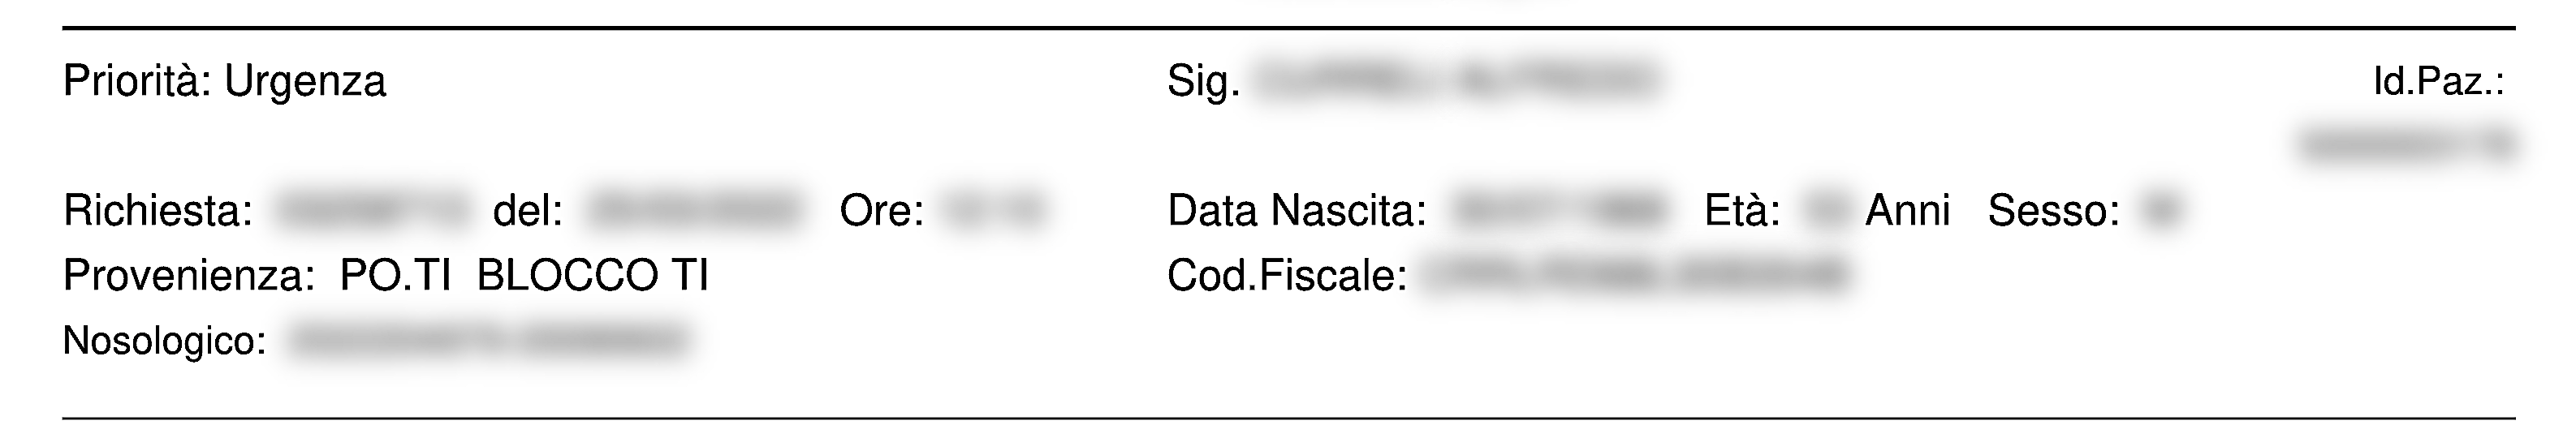
\includegraphics[width=.99\columnwidth]{images/sezione_anagrafica.png}
	\caption{\textit{Sezione anagrafica che mostra la priorità e le informazioni sul paziente}}
	\label{fig:header}
\end{figure}
\bigskip
\newline
La presenza di queste informazioni consente di verificare che il referto inserito nel sistema sia effettivamente del paziente selezionato, prevenendo cosi erronea associazione.

\newpage
\subsection{Il contenuto del referto}
Nel cuore del referto è collocato il risultato dell'analisi, che varia a seconda dell'obbiettivo del test. L'implementazione attuale è progettata per trovare ed estrarre le tabelle antibiogramma. 

\begin{figure}[h!]
	\centering
	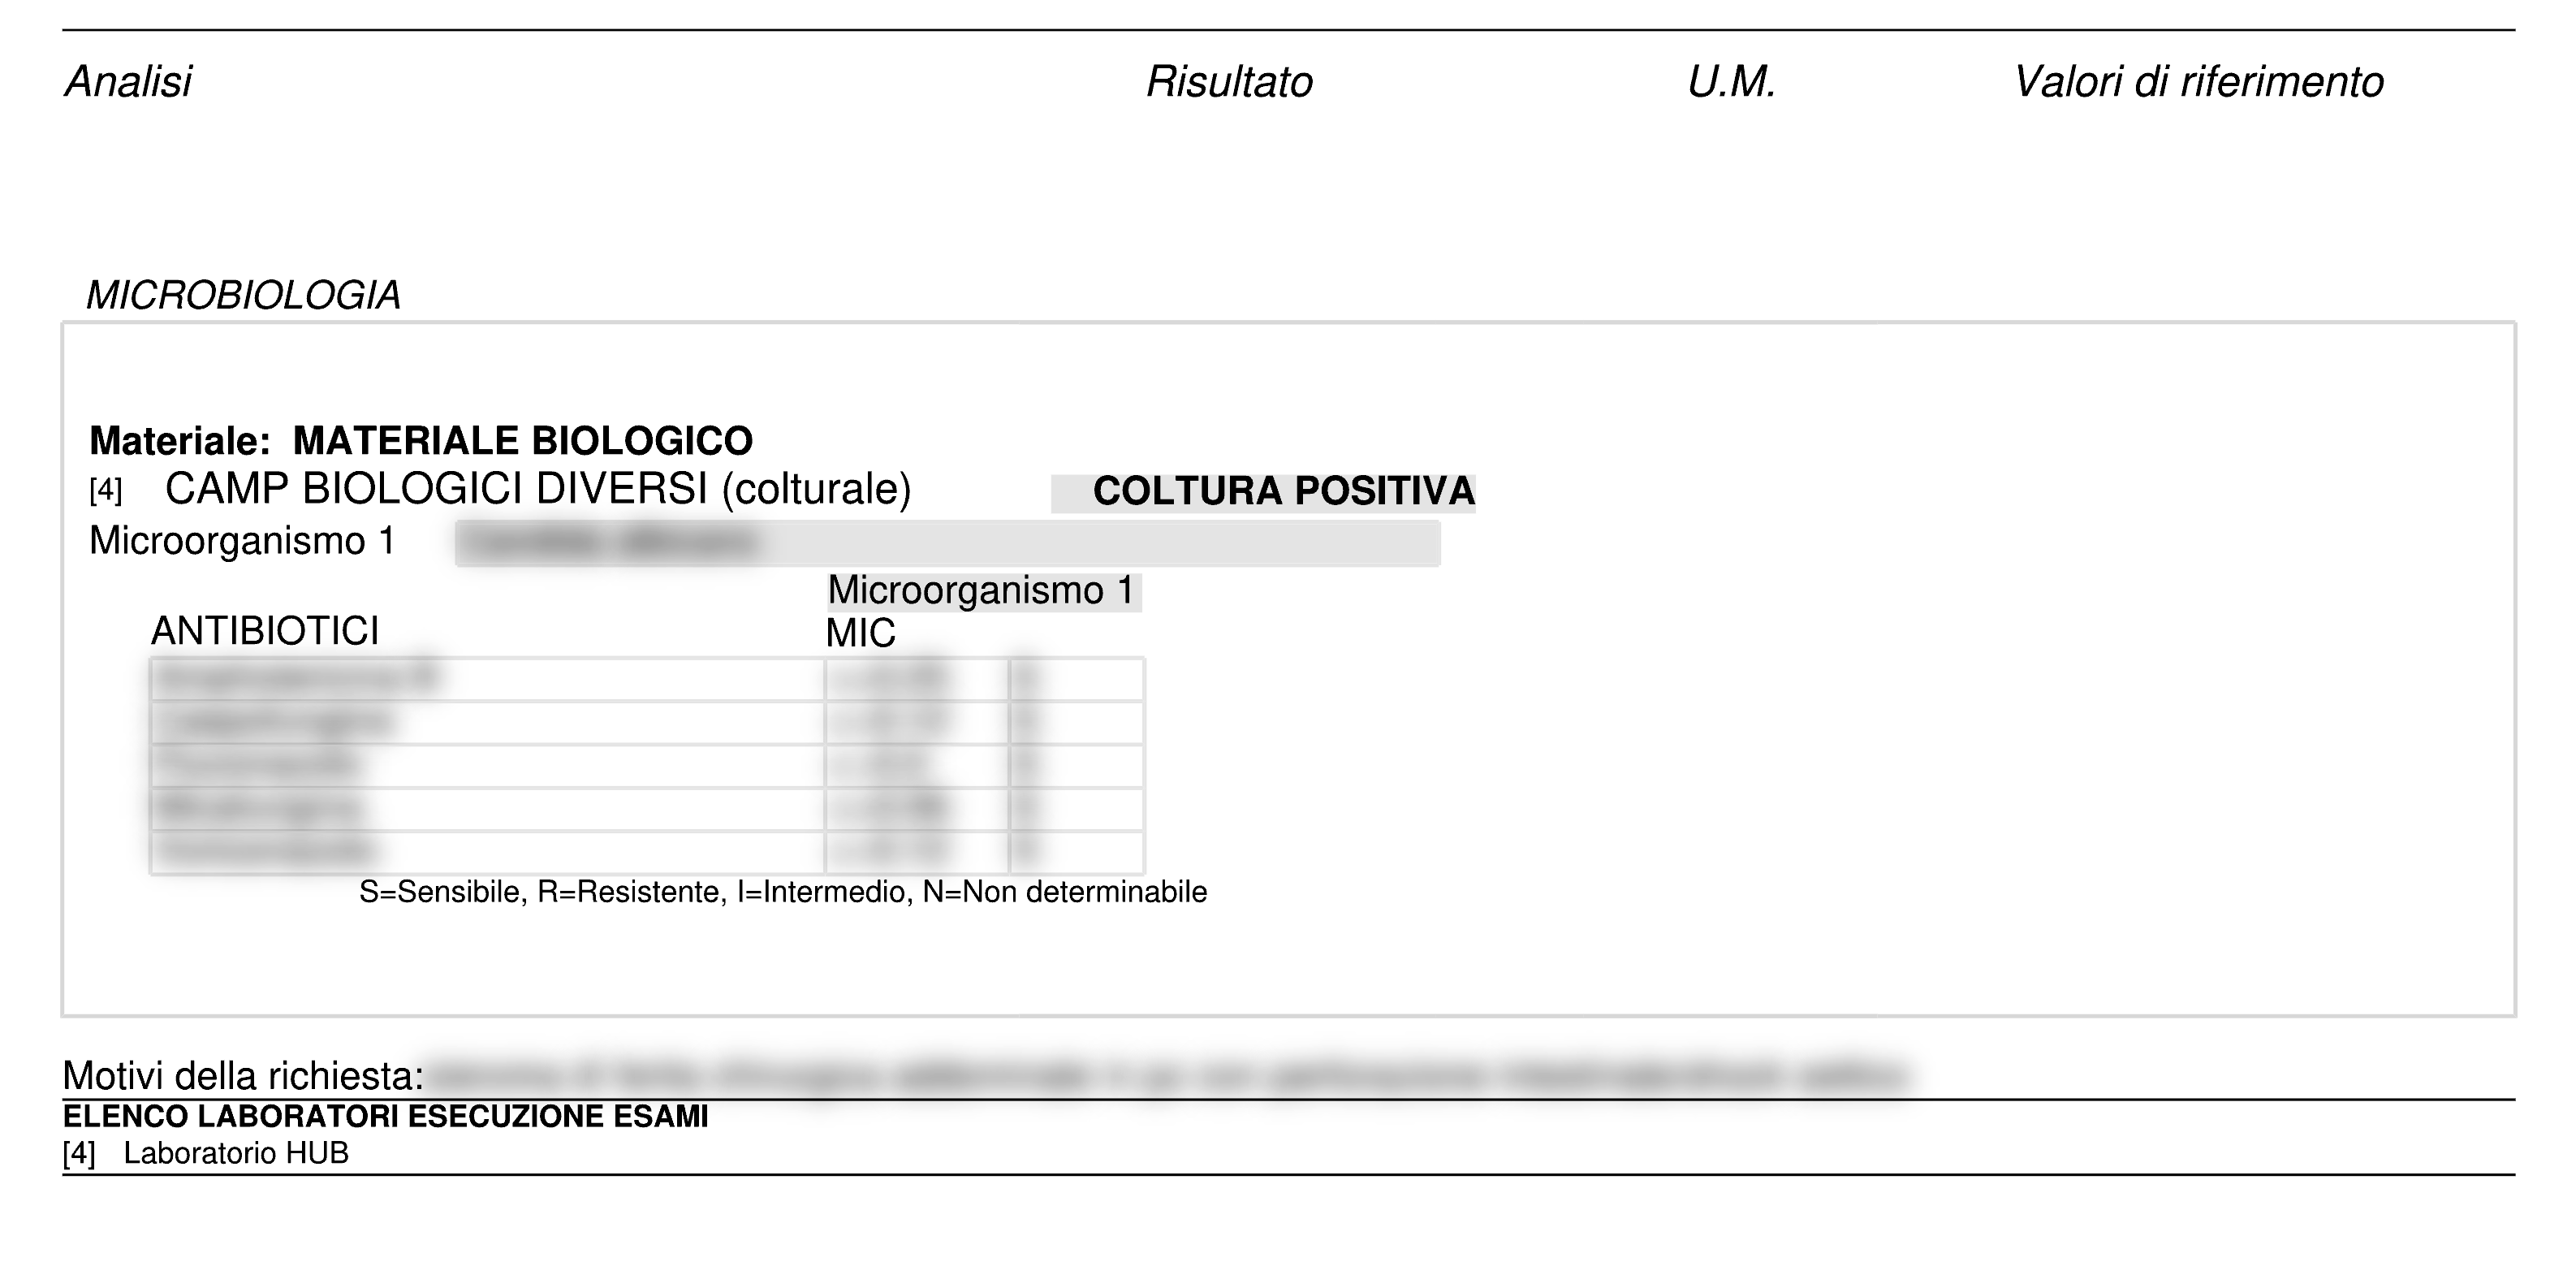
\includegraphics[width=.99\columnwidth]{images/content.png}
	\caption{\textit{Un antibiogramma valido per l'estrazione}}
	\label{fig:content}
\end{figure}
\bigskip
Nei referti validi, è presente una o più tabelle antibiogramma costituita da un minimo di tre colonne e un massimo indefinito ma solitamente non più di sette (una per gli antibiotici e due per ogni microrganismo fino a tre).
La prima colonna, comune a tutti i microrganismi a cui la tabella fa riferimento, indicano l'antibiotico testato e valori risultanti.
Segue la colonna la cui intestazione riporta la parola "MIC", che indica la "Minima Concentrazione" ossia la concentrazione più bassa (solitamente espressa come $\mu$g/mL ) per cui un determinato antibiotico è capace di inibire la crescita del microrganismo associato.
Dopo il MIC segue la colonna che rappresenta la sensibilità del microrganismo all'antibiotico testato con un set di valori definiti nella legenda posta sotto la tabella.
L'unione del microrganismo, gli antibiotici e relativi mic e sensibilità forma l'antibiogramma per il microrganismo in questione.


\subsection{Il piè di pagina}
Infine, il piè di pagina, che contiene informazioni sulla firma del documento, la relativa data e l'ora. Inoltre è presente un codice  che identifica il referto negli altri sistemi del policlinico.

\begin{figure}[h!]
	\centering
	
\includegraphics[width=.99\columnwidth]{images/footer.png}
	\caption{\textit{Piè di pagina (Footer)}}
	\label{fig:footer}
\end{figure}
\bigskip
\newpage

\section{Tipologie di referti}
Nell'ambito di questa tesi possiamo distinguere 5 tipologie di referti a seconda del loro contenuto:
\begin{itemize}
	\item Singolo Antibiogramma
	\item Antibiogramma multiplo
	\item Antibiogramma singolo multi-pagina
	\item Antibiogramma multiplo multi-pagina
	\item Referto senza tabelle
\end{itemize}
\bigskip
La prima tipologia è costituita da un singolo microrganismo seguito da una tabella con sole tre colonne, strutturate come descritto nel paragrafo 2.1.3, la figura \ref{fig:content} mostra nel dettaglio una tabella ad antibiogramma singolo.
 
L'antibiogramma multiplo invece presenta più microrganismo accorpati nella stessa tabella, pertanto avremmo una sola colonna per l'antibiotico ma un susseguirsi di colonne MIC-Sensibilità per ciascun microrganismo.
Le tabelle multipagina costituiscono una variazione rara ma non impossibile delle prime due tipologie, presentando le tabelle fisicamente divise fra una o più pagine.

\subsection{La sorgente dei dati}
I PDF dei referti sono generati tramite una libreria software chiamata "iText" che riceve in ingresso i dati degli antibiogrammi, sorge dunque spontanea la domanda: 
\begin{quotation}
  "Perchè non aggirare il referto e prelevare i dati dalla sorgente?"
\end{quotation}
Purtroppo i sistemi informatici del policlinico sono isolati e non di facile modifica, soprattutto a livello legale. Un eventuale alterazione del prodotto software designato implicherebbe un eventuale perdita di supporto dalla casa madre e problemi di privacy. Oltretutto potrebbe essere necessario inserire referti non generati dallo specifico programma utilizzato in un determinato reparto.





\chapter{Il PDF e l'Estrazione delle informazioni}
Prima di poter estrarre dati utili dai documenti PDF è necessario operare delle trasformazioni o delle rappresentazioni, dato che, per natura del PDF non vi sono dei dati utili al nostro scopo direttamente leggibili.

\section{Cosa sono i PDF?}
PDF è un acronimo che sta per \textit{Portable Document Format}, è un formato standard creato nel 1993 allo scopo di rappresentare documenti testuali o con immagini indipendentemente dall'hardware o dal software che usato per generare o visualizzare il documento stesso. I file costruiti in questo formato sono rappresentati tramite una sequenza di caratteri ASCII\footnote{Codice standard di codifica dei caratteri americano, uno standard \textit{de-facto} utilizzato nei computer IBM}, all'interno possiamo individuare quattro strutture:

\begin{itemize}
	\item Header
	\item Body
	\item Cross-Reference Table
	\item Trailer
\end{itemize}
Ciò che viene presentato visivamente all'utente è contenuto nella sezione \texttt{body} del PDF, su questo flusso di caratteri si opera per ottenere le informazioni volute.
\newpage
\section{Tecniche di estrazione}
Le tecniche di estrazione sono principalmente due:
\begin{itemize}
	\item Conversione in formati testuali
	\item Lettura diretta del flusso \texttt{Body}
\end{itemize}

Nel primo caso si cerca di convertire (tramite librerie o servizi appositi) il documento in un file di testo dove poter effettuare l'estrazione. Questo metodo è stato scartato durante i test d'implementazione preliminari per via del risultato insoddisfacente, difatti i tentativi di conversione (con strumenti già esistenti e librerie dedicate) non riuscivano a convertire le tabelle in testo ma venivano generate delle immagini. 
Non è stato possibile utilizzare librerie dedicate all'estrazione di tabelle poiché gli antibiogrammi hanno una posizione fissa.
Nel secondo caso la realizzazione di un prodotto completo avrebbe richiesto studi molto più lunghi e fuori dallo scopo della tesi.
\section{La libreria utilizzata}
In un primo momento si è tentato di utilizzare la stessa libreria responsabile della generazione dei documenti, ma limitazioni di licenza e funzionalità hanno favorito la concorrente open-source Apache PDFBox che si è rivelata oltretutto più versatile e adatta allo scopo prefissato.
\section{L'approccio iniziale e le problematiche}
Il primo approccio si è basato sulla semplice estrazione del testo linea per linea dai referti con l'applicazione di specifiche regex. 
Avendo inizialmente soltanto un referto su cui effettuare i test non è apparso subito l'evidente problema sorto in seguito con gli antibiogrammi multi-microrganismo.
L'algoritmo di estrazione era dunque costituito dai seguenti passaggi:
\begin{enumerate}
\item Scorrere la lista fino a trovare la stringa corrispondente alla parola "Microrganismo 1" seguito dal nome del microrganismo
\item Scorrere di 2 posizioni (equivalenti a saltare la riga "Microrganismo 1" e "ANTIBIOTICO MIC")
\newpage
\item Verificare ed estrarre le informazioni riguardo alla riga della tabella tramite la seguente regex:
\begin{figure}[h!]
	\centering
	
\includegraphics[width=.99\columnwidth]{images/regex.png}
	\caption{\textit{Regex per l'estrazione delle righe della tabella}}
	\label{fig:content_multi_1}
\end{figure}
\item Ripetere fino all'arrivo della riga contenente la legenda.
\end{enumerate}

Per poter estrarre le informazioni da tabelle con più microrganismi è possibile modificare la regex ripetendo la seconda riga (la parte col gruppo MIC e Sensibilità) quante volte sono i microrganismi individuati.
Questa soluzione però fallisce nel caso di coppia di celle vuote (che significa analisi antibiotica non condotta per tale microrganismo).
\newline
\begin{figure}[h!]
	\centering
	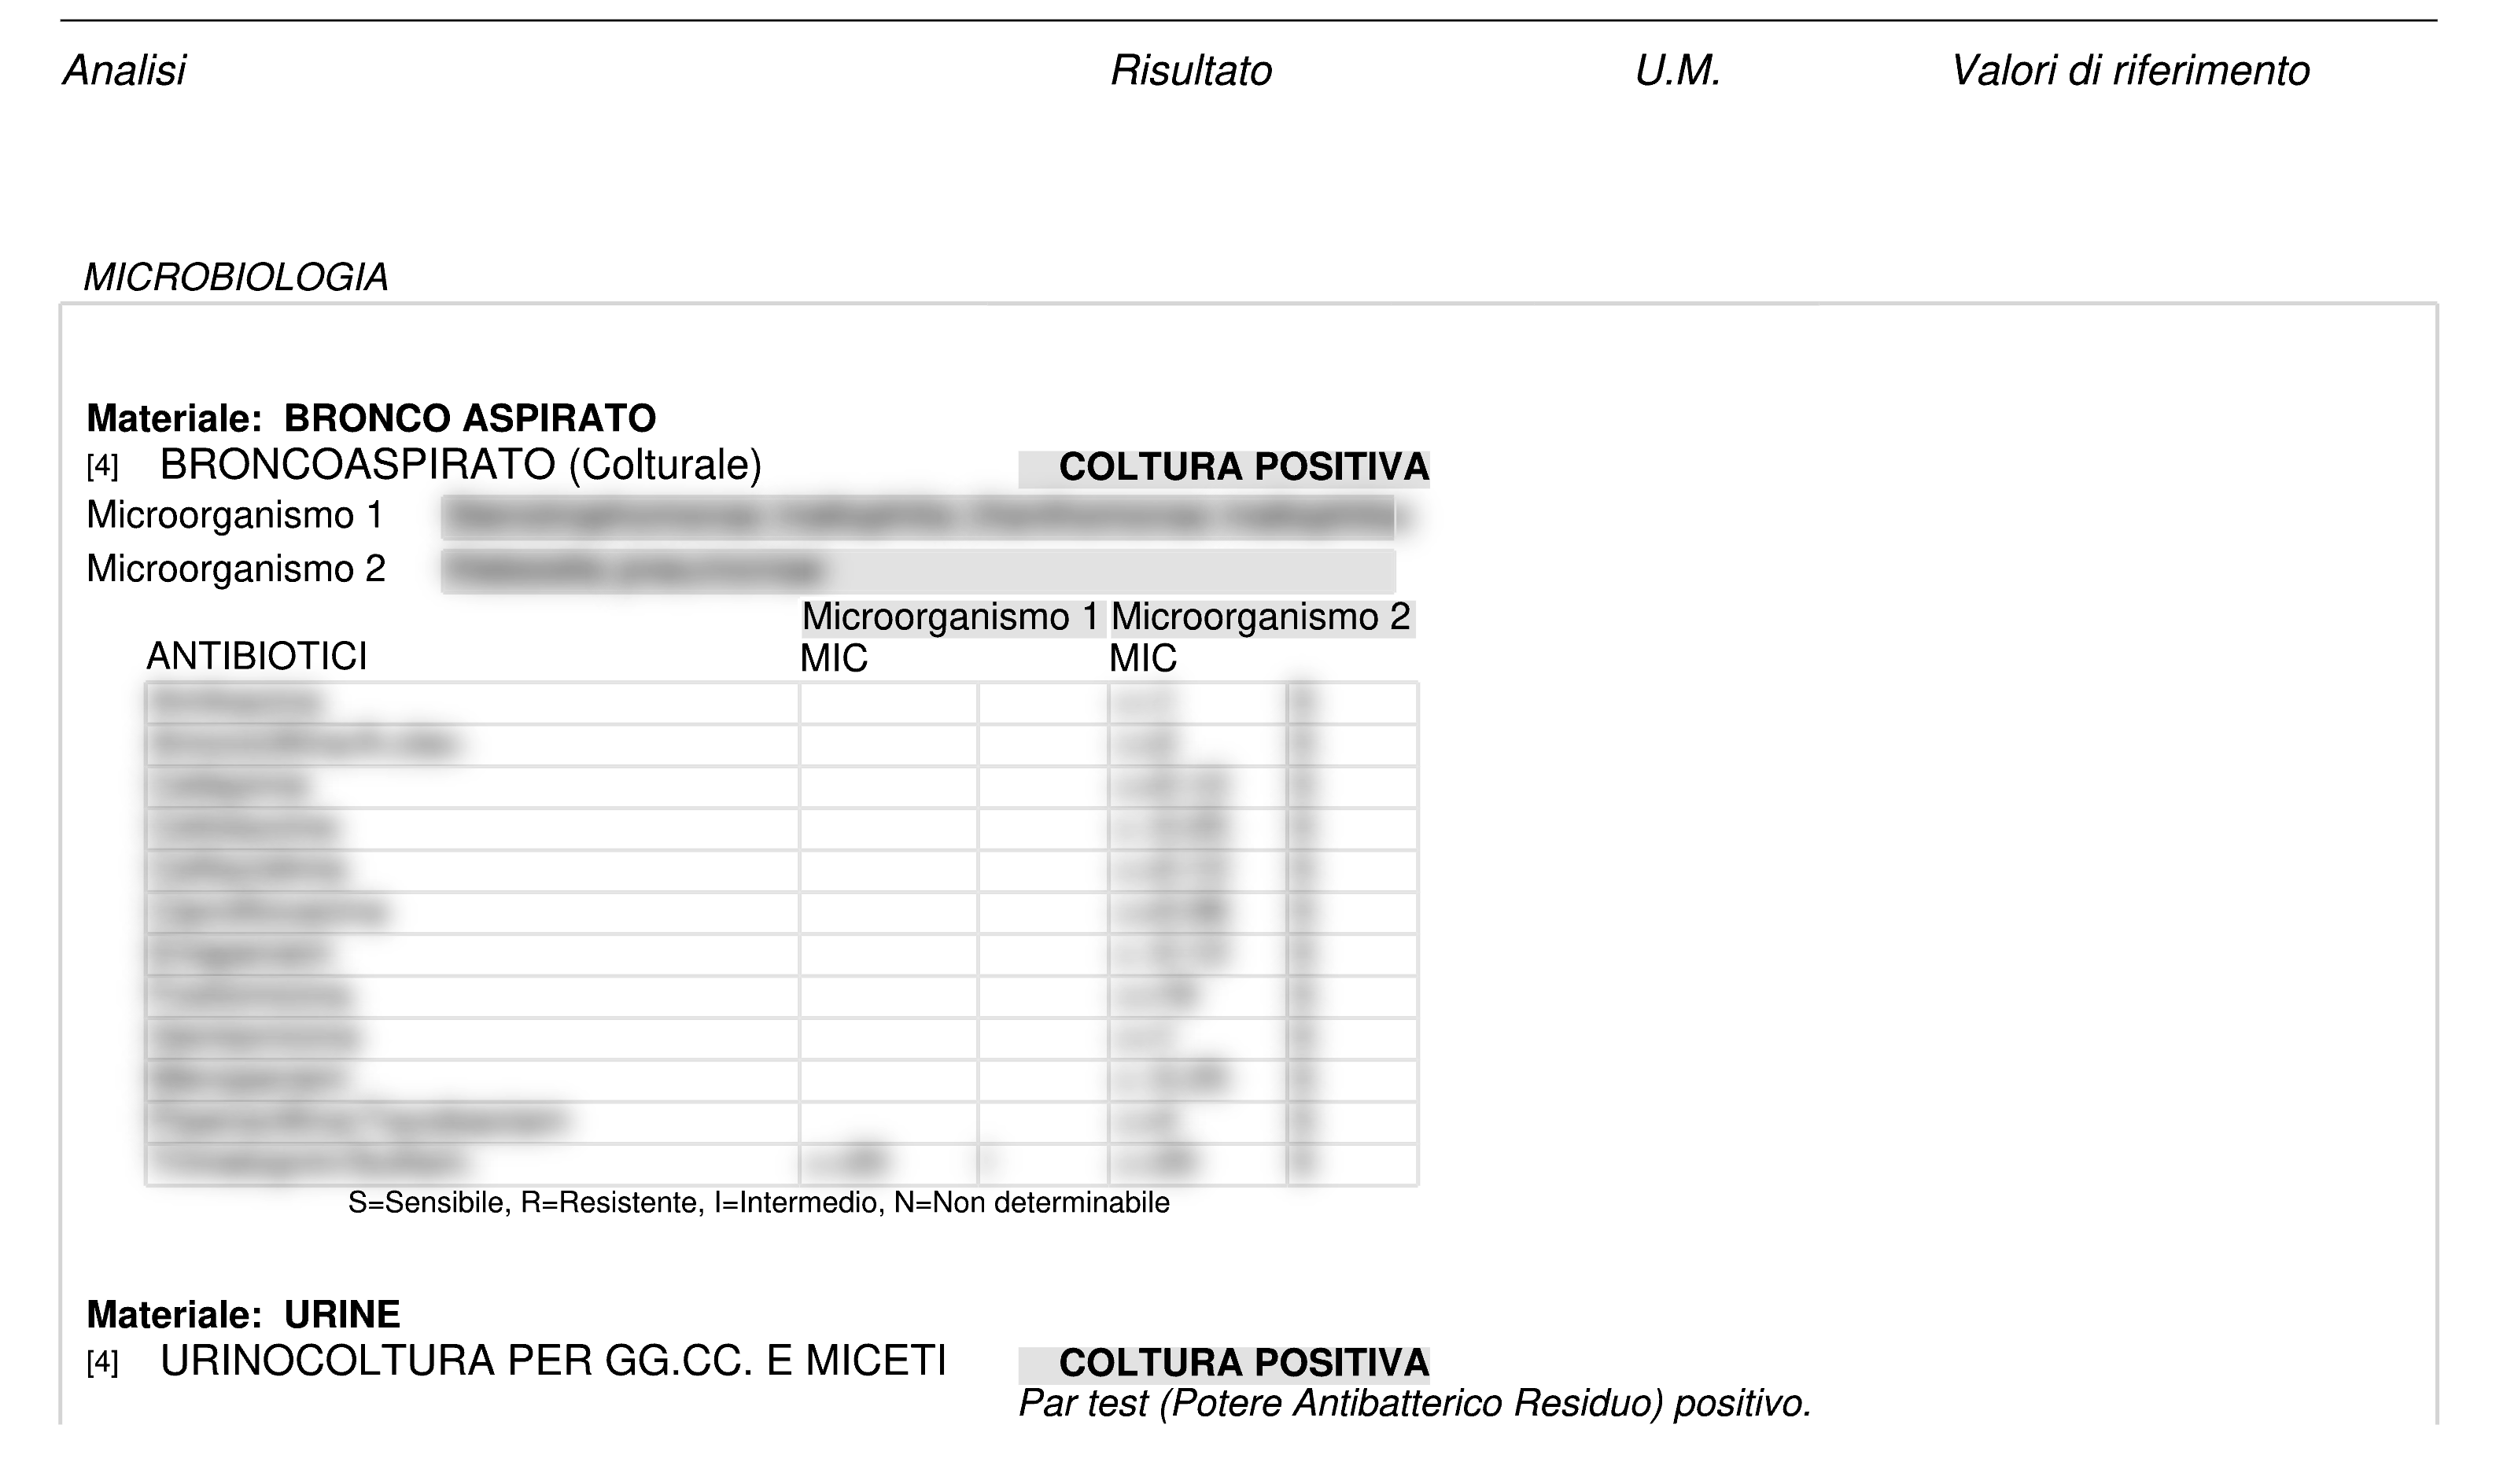
\includegraphics[width=.99\columnwidth]{images/content_multi_p1.png}
	\caption{\textit{Tabella con più microrganismi}}
	\label{fig:content_multi_1}
\end{figure}
\newline
Per esempio, nella tabella mostrata nella figura \ref{fig:content_multi_1} soltanto l'ultima riga potrà estrarre dei risultati validi tramite modifica delle regex, che risulterebbe la seguente:
\begin{figure}[h!]
	\centering
	
\includegraphics[width=.99\columnwidth]{images/regex_2.png}
	\caption{\textit{Regex per l'estrazione delle righe della tabella}}
	\label{fig:content_multi_1}
\end{figure}
Dove \textit{NR\_MICRO} è da sostituire col numero di microrganismi.
\section{Il secondo approccio}
Il secondo approccio, che apporta la modifica più significativa, rivede completamente la logica di estrazione e aggiunge delle modifiche alla libreria PDFBox.
Il concetto fondamentale di quest'approccio è un'estrazione "ibrida" ossia si ricerca l'inizio della tabella come nel metodo precedente, ma l'estrazione dei dati vera è propria viene effettuata calcolando la posizione delle varie celle.
\newline
Infatti, anche se la posizione e la dimensione della tabella non è costante, le celle invece lo sono, permettendo un calcolo preciso della loro posizione e conseguente estrazione.
\subsection{Modifiche alla libreria}
Per ottenere la posizione degli elementi si è proceduto ad estendere la classe \textit{PDFTextStripper} della libreria aggiungendo prima una lista di oggetti di tipo \texttt{<string, List<TextPosition>}, ogni oggetto di questa lista è composto da una coppia chiave-valore in cui la chiave è una qualsiasi parola estratta e la chiave è una lista di posizioni in cui ogni lettera ha una sua coordinata.
Come seconda cosa è stato modificato il metodo \textit{writeString} in modo che inserisse nella lista prima citata queste nuove informazioni lasciando però inalterato il resto delle istruzioni.
\newline
\subsection{Localizzazione delle celle}\label{Algoritmo finale}
Una volta generate queste informazioni è possibile rappresentare l'algoritmo come segue:
\begin{enumerate}
	\item Si effettua una prima ricerca della tabella in modo analogo al metodo precedente
	\item Si continua a scorrere la lista e si tiene traccia del numero di microrganismi presenti nella tabella trovata
	\item Finita l'enumerazione dei microrganismi, si inizia a scorrere la nuova lista della classe modifica fino a trovare la parola chiave "ANTIBIOTICI", seguita da tante stringhe "MIC" quanti sono i microrganismi
	\item L'elemento puntato dalla lista sarà il nome dell'antibiotico, da qui si calcolano le dimensioni e le posizioni delle celle MIC e Sensibilità
	\item Definiamo tre "regioni" (dei rettangoli in cui operare), una per estrarre il nome dell'antibiotico alla linea selezionata, una per quella successiva e una per la legenda
	\item Si tenta la prima estrazione del testo, seguita poi, per ogni microrganismo dai seguenti passi:
	\begin{enumerate}
		\item Si calcola la cella MIC le cui coordinate saranno: distanza colonna antibiotico $ + 156 + $ (n° microrganismo)$*42$
		\item Discorso analogo per la cella Sensibilità che ha coordinate: distanza colonna MIC $ + $ (n° microrganismo) $*30*$
		\item Vengono definite altre due regioni, si tenta l'estrazione e si inseriscono le informazioni raccolte nell'antibiogramma
		\end{enumerate}
		\item Fatto questo, si scorre la lista delle parole fino a trovare o la legenda (che indica la fine della tabella e dell'estrazione) o il prossimo antibiotico (si confronta il testo con il dato estratto prima). Nel secondo caso si ferma lo scorrere della lista e si riparte del punto 4.
\end{enumerate}
		
Questi 7 passaggi sono ripetuti per ogni pagina del PDF, ed è una soluzione quasi definitiva ma non esente da difetti. Ma cosa succede se ci sono più tabelle per pagina? Semplicemente viene rilevata soltanto la prima tabella e le successive vengono ignorate.
\section{L'approccio definitivo}
Al fine di ridurre la complessità del codice, è stato effettuata una riorganizzazione e parziale riscrittura che ha portato alla suddivisione del codice in due sotto-funzioni principali: la rilevazione delle tabelle e l'estrazione.
La rilevazione delle tabelle effettua un controllo pagina per pagina e differentemente da prima la ricerca continua fino all'indice delle line che rappresenta il fine pagina.
L'estrazione delle tabelle funziona in modo analogo alla soluzione precedente, con l'unica differenza che viene invocata con gli indici di inizio e di fine della tabella su cui operare. 
Questi piccoli accorgimenti permettono una migliore lettura del codice e di estrarre tutte le tabelle presenti, non soltanto la prima, rendendo l'algoritmo più preciso.
Non sono ancora stati testati referti con tabelle divise su più pagina perché non sono stati forniti esempi, si pensa che esistano perché nei campioni forniti alcuni presentano informazioni su materiale d'estrazione o componenti grafici in pagine differenti rispetto alla posizione della relativa tabella. Un esempio è la figura \ref{fig:content_multi_1} dove avviene proprio l'esempio del materiale; infatti, la tabella relativa si trova nella seconda pagina (figura \ref{fig:content_multi_2})
\newpage
\begin{figure}[h!]
	\centering
	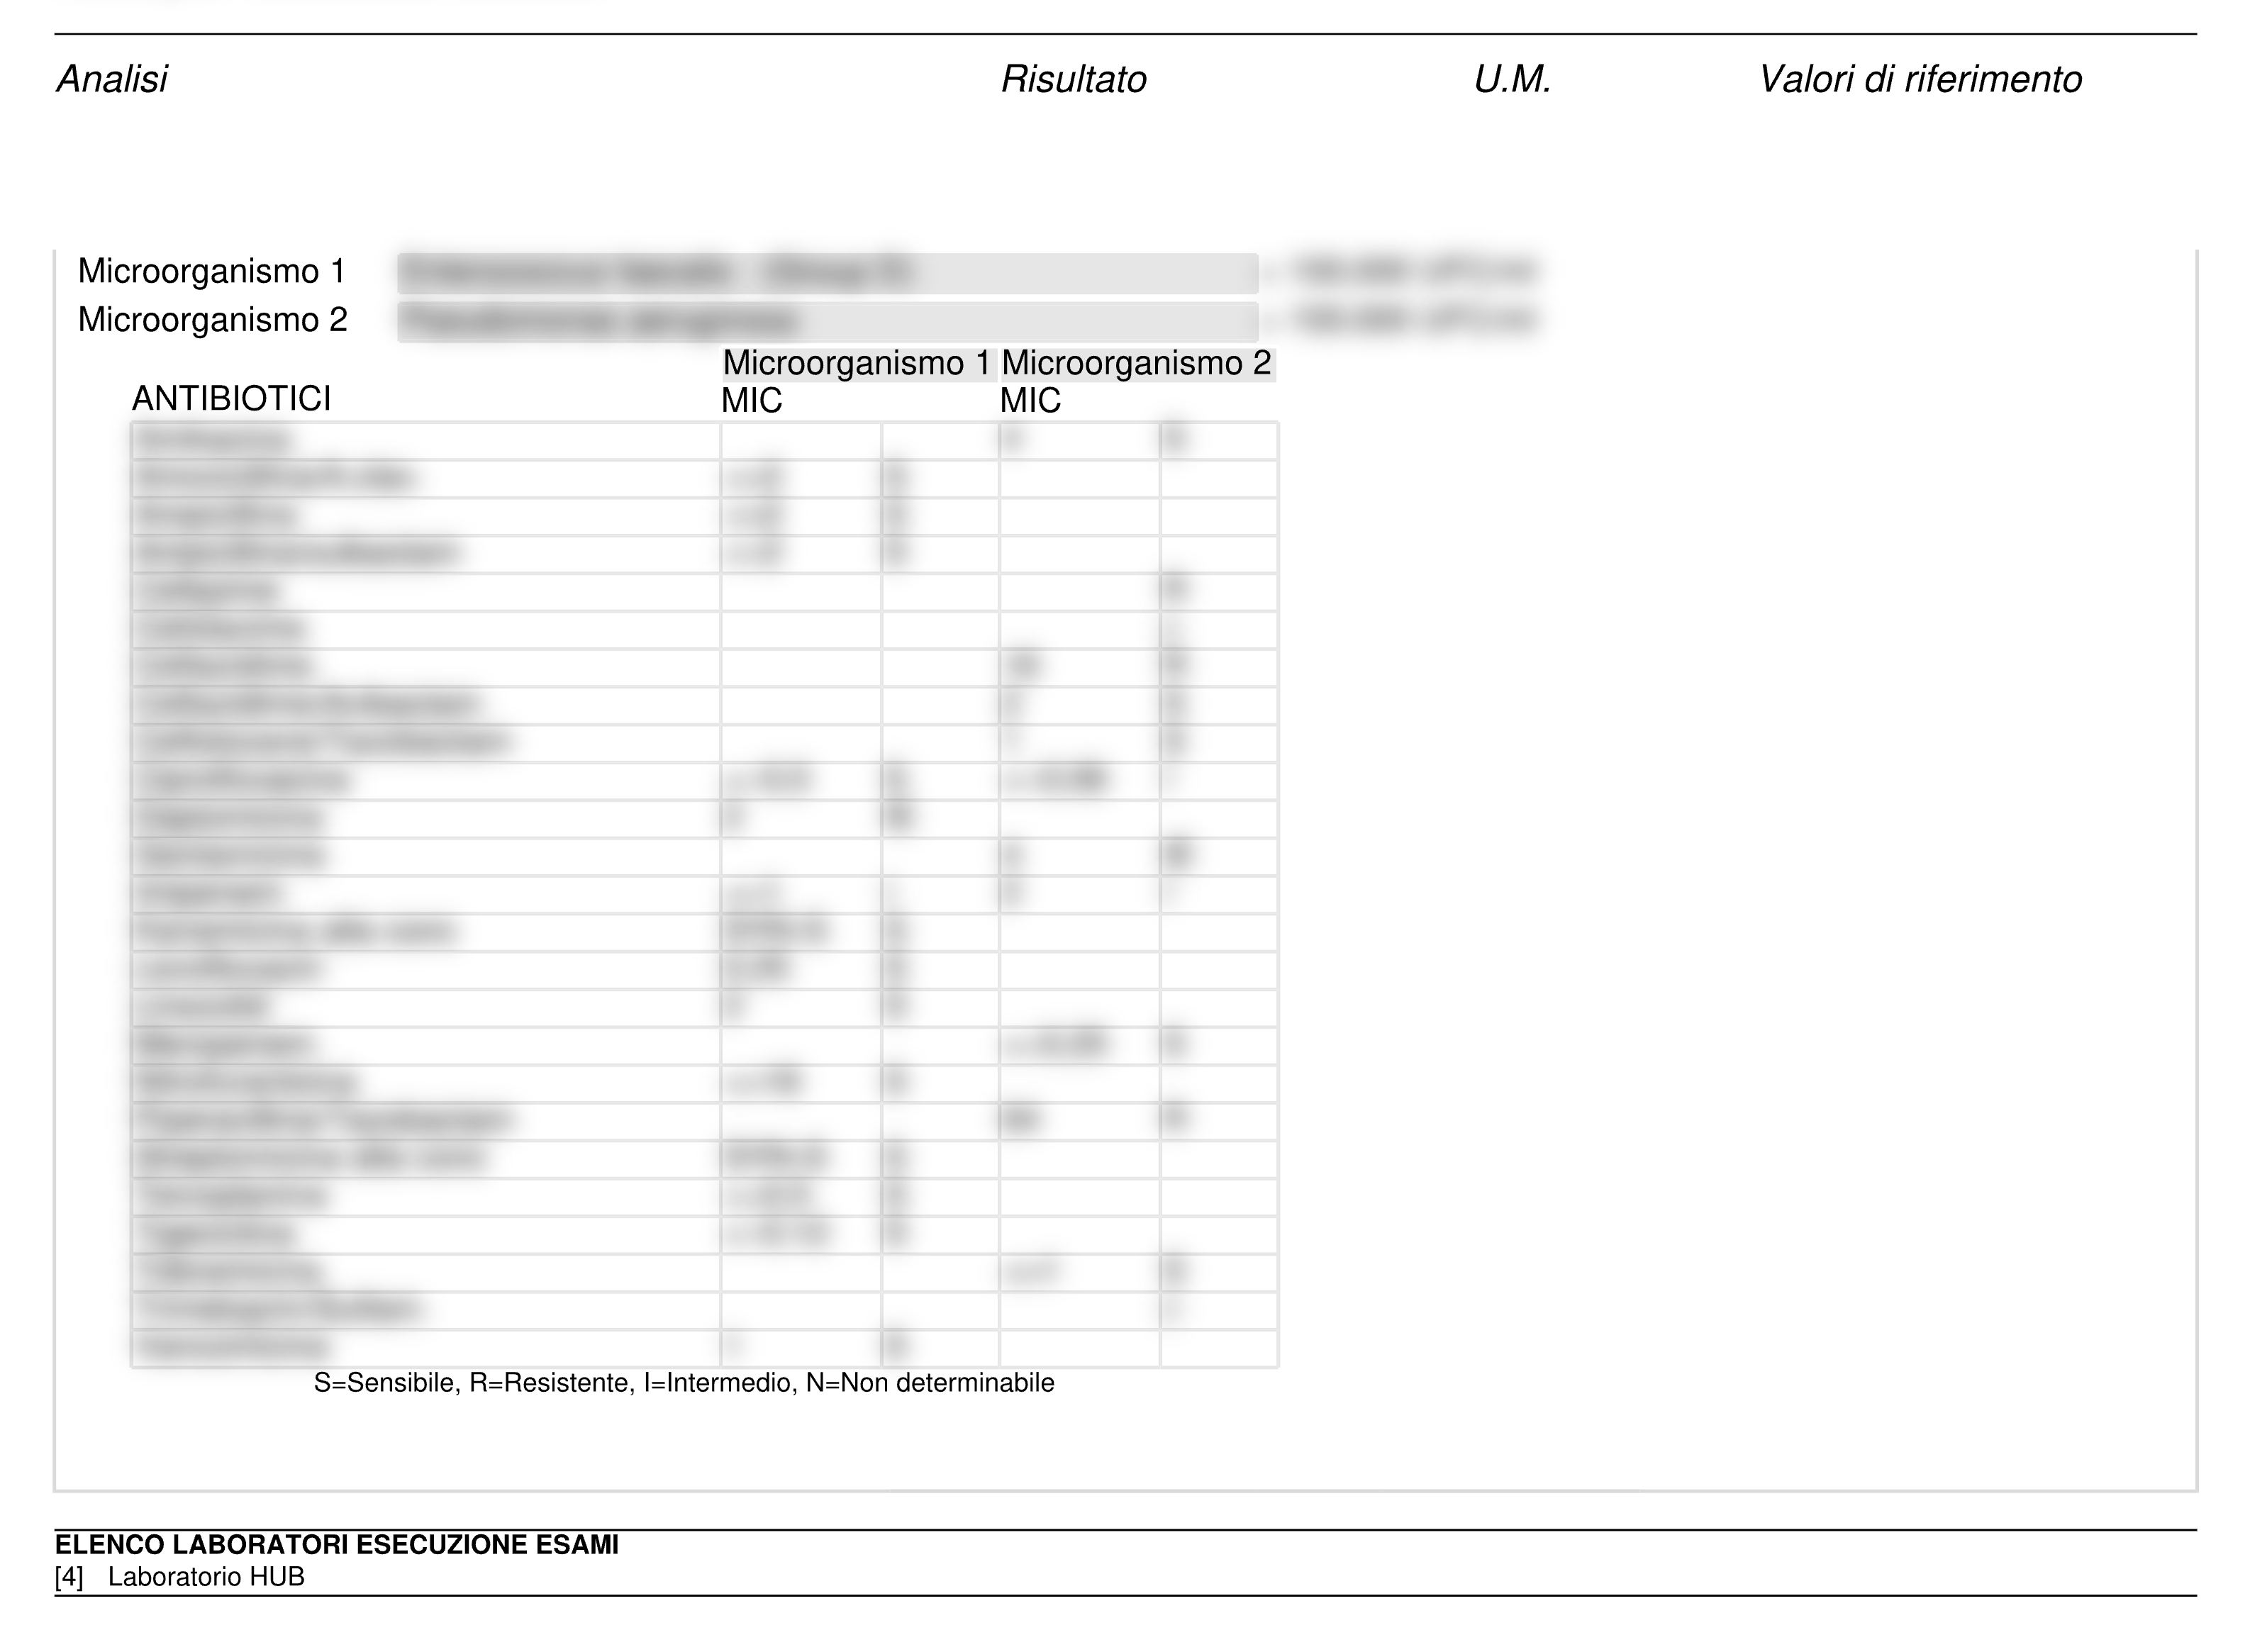
\includegraphics[width=.99\columnwidth]{images/content_multi_p2.png}
	\caption{\textit{}}
	\label{fig:content_multi_2}
\end{figure} 

La tabella in questione non presenta appunto il materiale su cui è basata l'analisi, poiché non è noto l'algoritmo utilizzato per dividere le informazioni si propone una soluzione aggiuntiva, da verificare una volta ottenuti campioni conformi, nella seguente forma algoritmica:
\begin{enumerate}
	\item Per ogni pagina, rimuovere le sezioni:
	\begin{enumerate}
		\item \textit{Intestazione} (fig. \ref{fig:header})
		\item \textit{Anagrafica} (fig. \ref{fig:content})	
		\item \textit{Piè di Pagina} (fig. \ref{fig:content})
	\end{enumerate}	
	\item Unire le pagina in una sola
	\item Procedere dal punto 1) dell'algoritmo proposto nel paragrafo \ref{Algoritmo finale}
\end{enumerate}
\newpage
\section{Risultati}
I risultati sono stati raccolti da due fonti: le mail scambiate con i medici e i feedback rilasciati nella relativa sezione inserita nel progetto per questa tesi (vedi \ref{label:modifiche_strutturali}).
Il sistema è stato giudicato ottimo sia per la semplicità che per la correttezza dell'implementazione, con una volontà da parte degli utenti di sfruttare il più possibile il sistema e trovare una soluzione agli impedimenti burocratici incontrati nella fase di distribuzione del progetto.






\chapter{Le modifiche al SIMIOR}
Per accomodare le nuove funzionalità è stato necessario fare delle modifiche strutturali al SIMIOR, spaziando dal database a classi di gestione dei dati interne al front-end del progetto.
\section{Modifiche strutturali}
Le modifiche fatte si possono raggruppare in tre punti:
\begin{itemize}
	\item Database
	\item Archivio Statico
	\item Front-End
\end{itemize}
Oltre al database che contiene i dati creati dagli utenti, il SIMIOR possiede dei dati "statici" che raramente richiedono una modifica, un esempio di questi dati sono i codici degli antibiotici definiti dal sistema ATC/DDD (Anatomical Therapeutic Chemical/Defined Daily Dose) o i codici dei microorganismi definiti dall'Istituto Superiore di Sanità.
Quando viene effettuato un inserimento di un antibiogramma (sia tramite la nuova funzionalità sia manualmente) il sistema effettua una ricerca in questo archivio statico per estrarre il codice relativo al microrganismo/antibiotico, ma inizialmente questi nomi erano in lingua inglese (sempre seguendo il sistema di origine dei dati) causando il fallimento dell'estrazione. Per ovviare a questo problema si è prima provveduto ad aggiornare l'archivio con la versione italiana e in secondo luogo aggiungendo la possibilità di avere un valore alternativo per casi particolari verificati in alcuni referti.
Che altro ho cambiato?
\newpage
\section{Implementazione FrontEnd}
L'utente può utilizzare la funzionalità recandosi nella sezione \textit{infezione, contaminazione o colonizzazione} di un qualsiasi ricovero, dove troverà una scheda contenente l'essenziale per poter allegare un referto e procedere con il caricamento.
\subsection{Localizzazione della funzionalità}
\begin{figure}[h!]
	\centering
	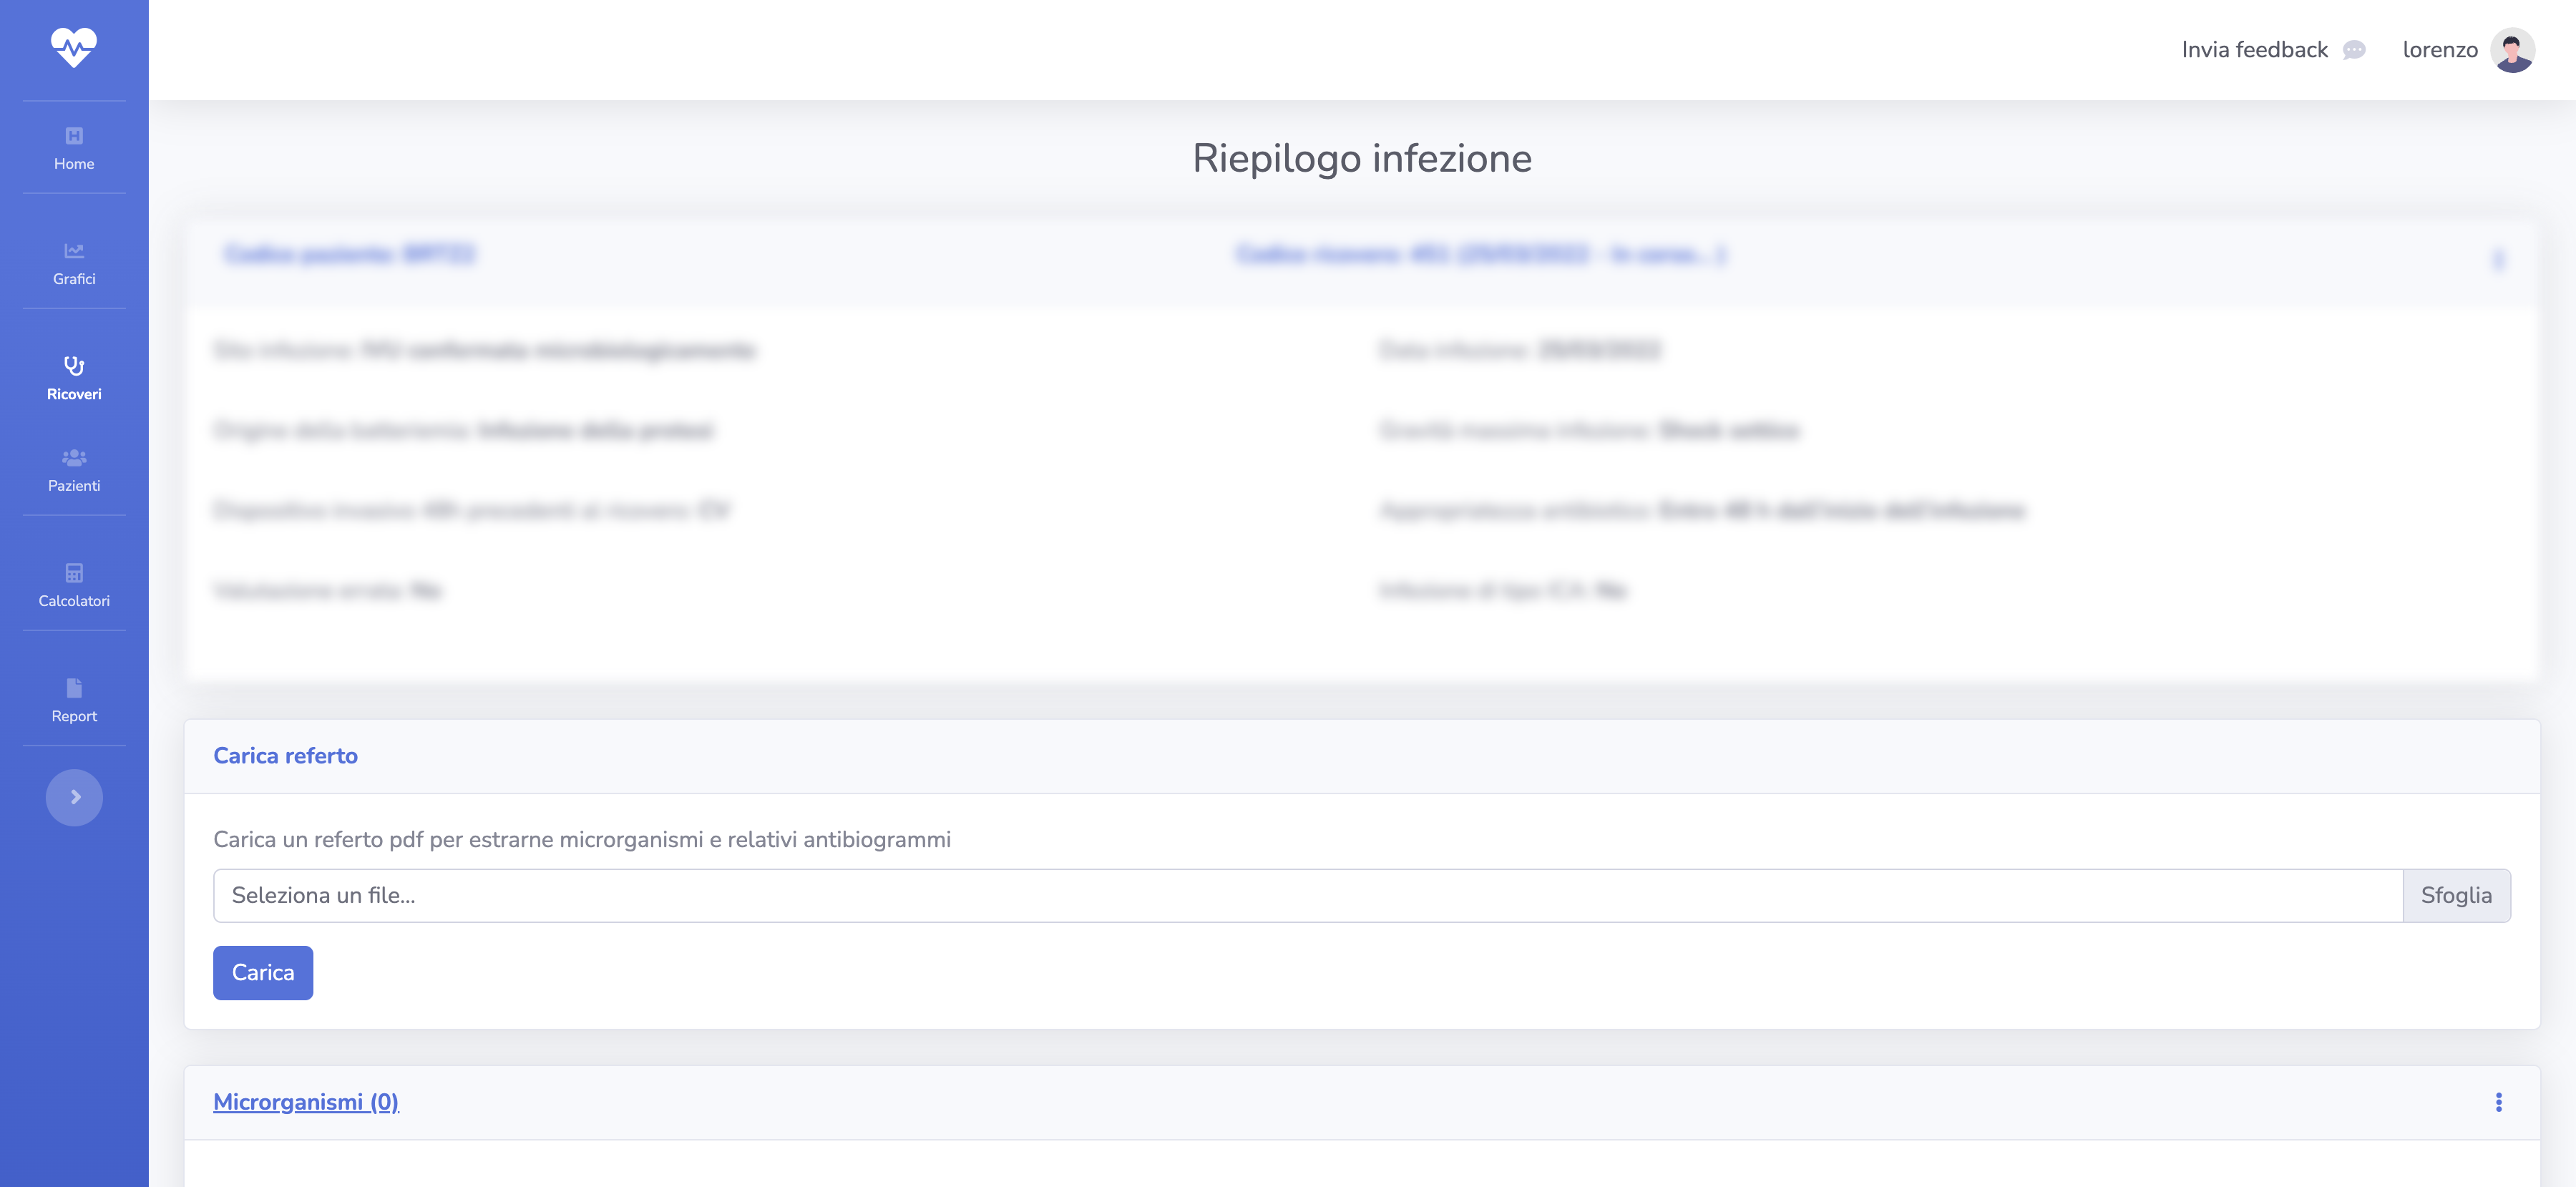
\includegraphics[width=.99\columnwidth]{images/feature_location.png}
	\caption{\textit{Scheda upload documento}}
	\label{fig:feature_location}
\end{figure}

La pressione del tasto \textit{"Sfoglia"} aprirà una schermata di dialogo gestita dal sistema che permetterà di selezionare il file determinato. Fatto questo l'utente procede alla pressione del tasto \textit{Carica} che lo porterà a una seconda pagina dove verranno mostrati i risultati dell'estrazione.
\subsection{La schermata dei risultati}

\begin{figure}[h!]
	\centering
	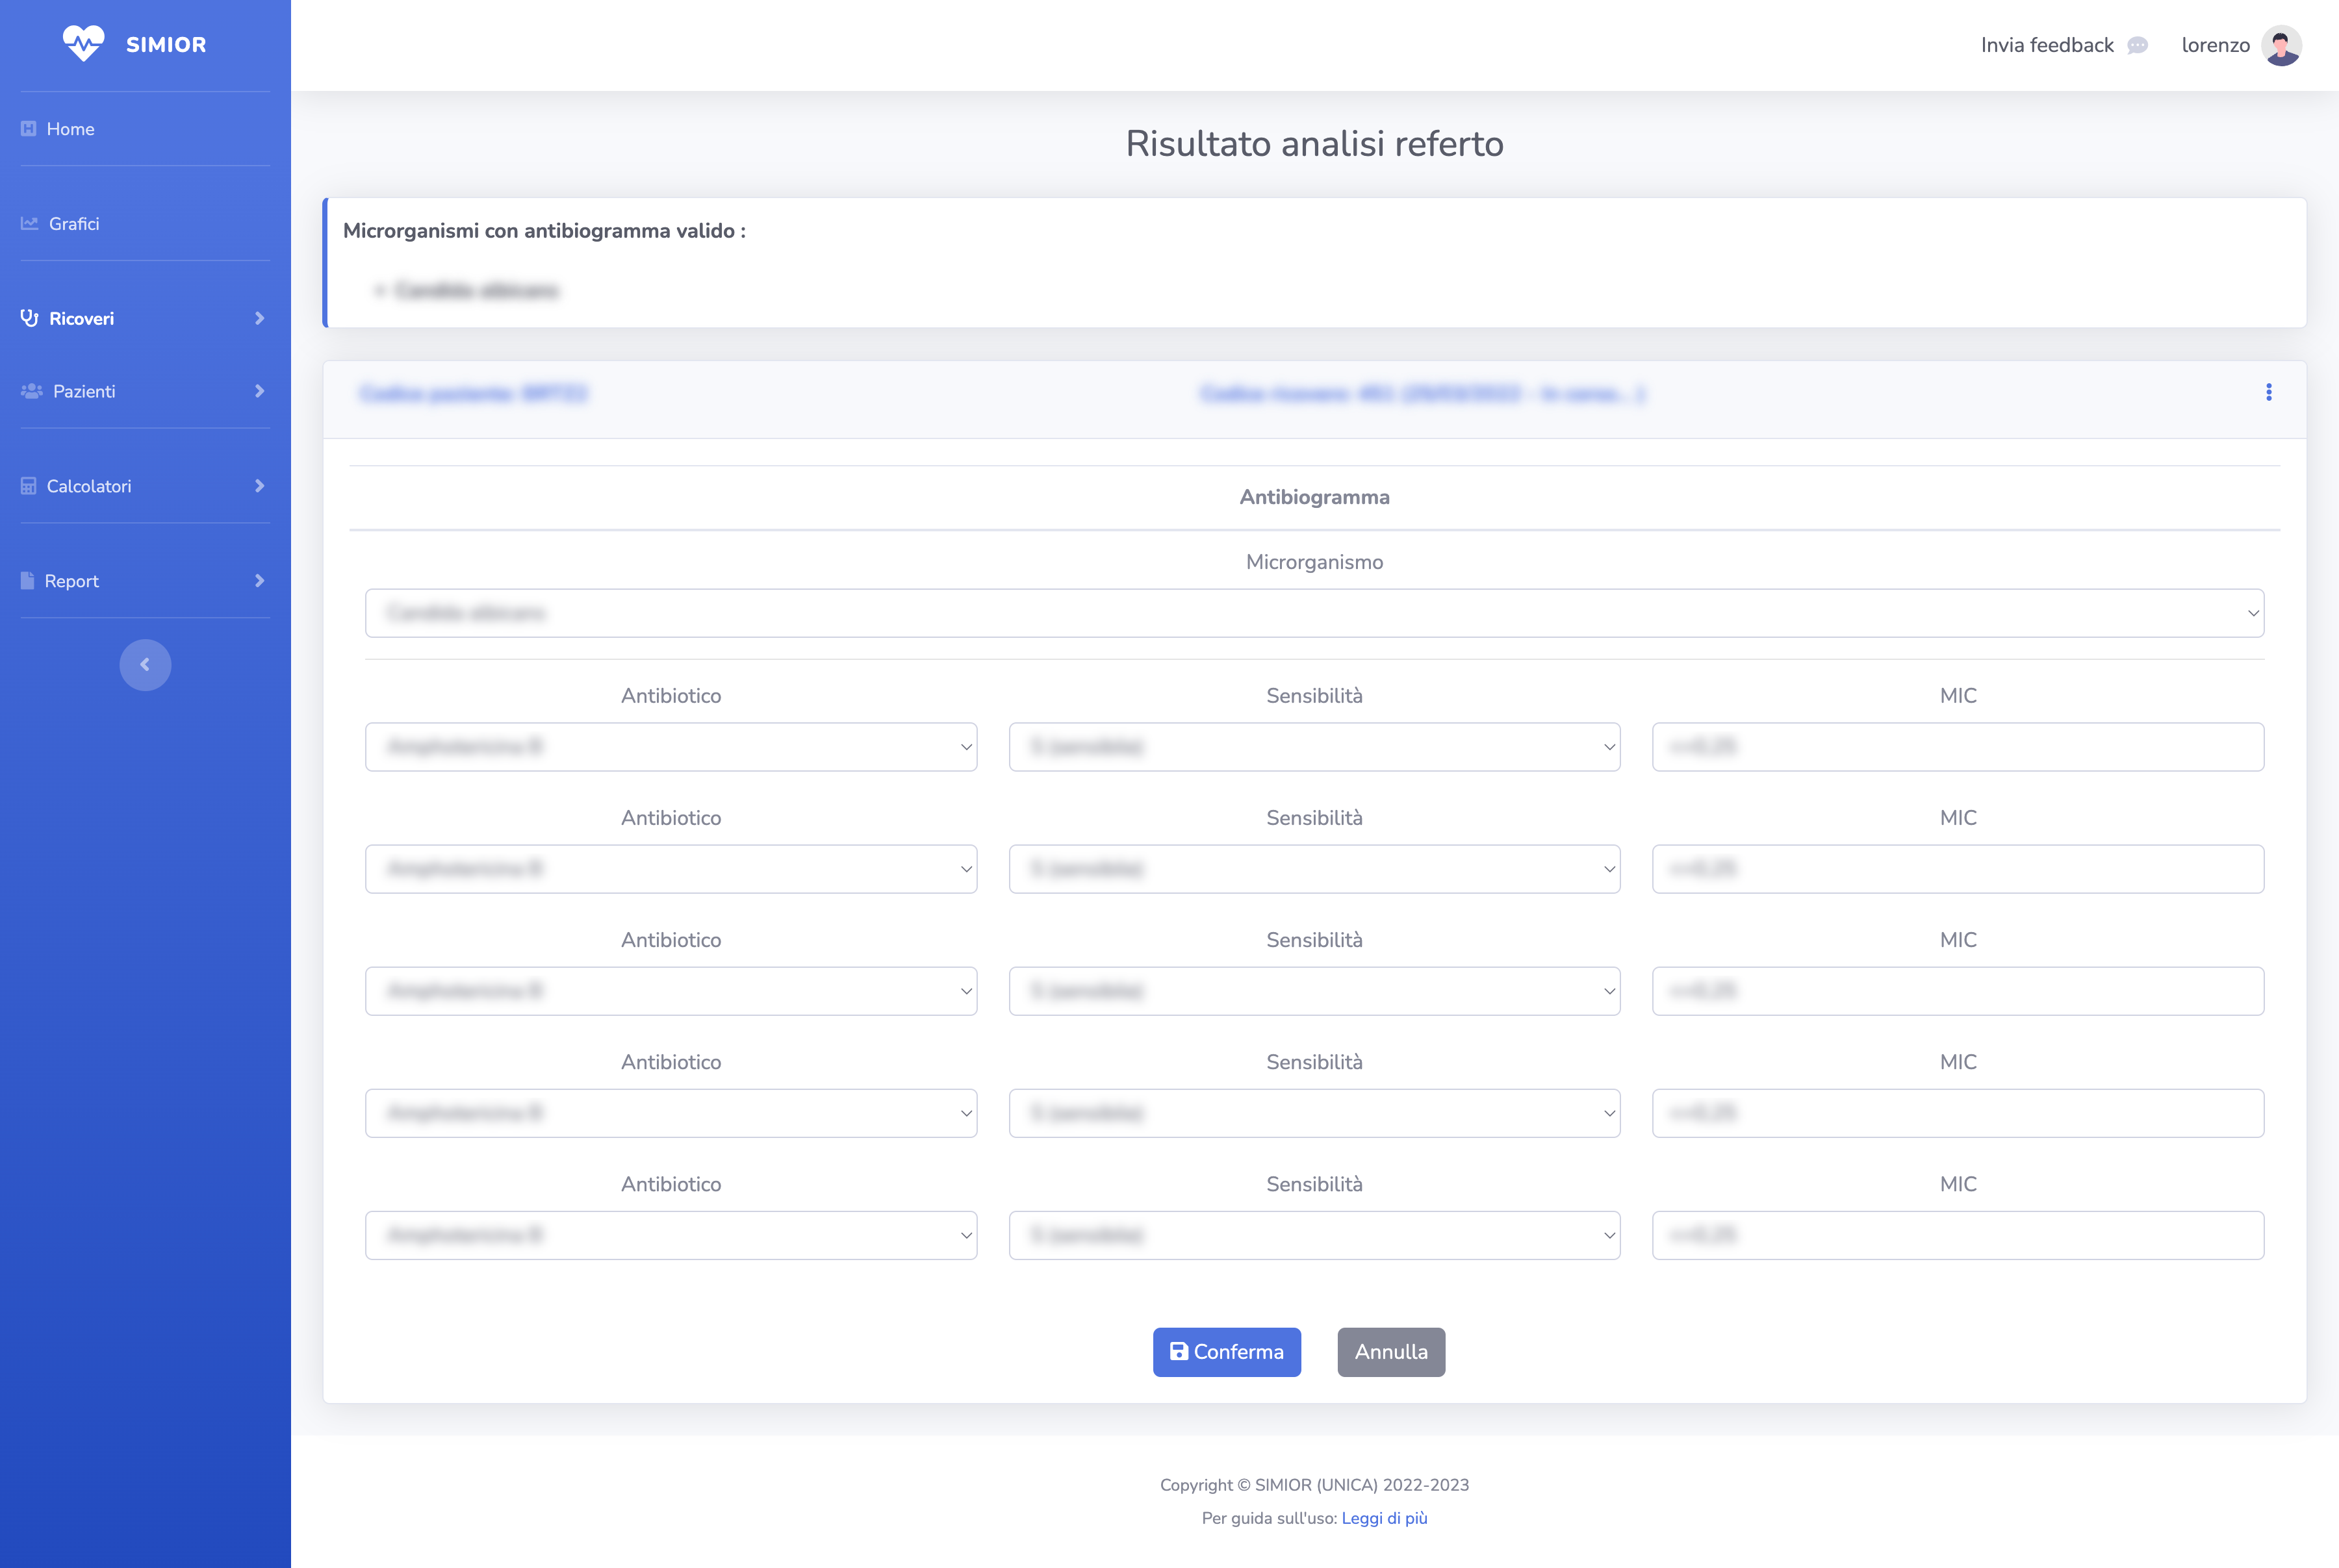
\includegraphics[width=.99\columnwidth]{images/extraction_result.png}
	\caption{\textit{Risultati estrazione}}
	\label{fig:extraction_result}
\end{figure}

\begin{figure}[h!]
	\centering
	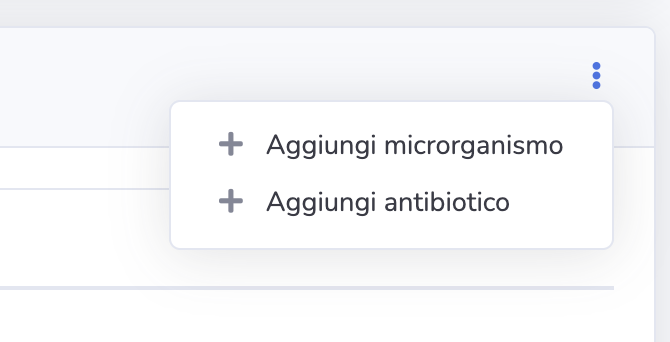
\includegraphics[width=.99\columnwidth]{images/new_object.png}
	\caption{\textit{Drop-down con le opzioni}}
	\label{fig:new_object}
\end{figure}

\chapter{Conclusioni}
\section{Non ne ho idea}
\bibliographystyle{plain}
\bibliography{biblio}


\end{document}
